\documentclass[11pt]{article}

\usepackage{epsfig}

\begin{document}

\begin{center}
{\Large \bf Building the Super-VMW CPU Meter}\\
{\tt http://www.deater.net/weave/vmwprod/meter/super.html}\\
by Vincent M. Weaver\\
18 May 2011
\end{center}


\section{Parts List}

\begin{tabular}{|c|l|c|c|}
\hline
Part No   &  Description    &  Quantity    &   Source \\
\hline
\hline

          &  LED Board                 & 1  & SVMW-Meter-LED-Board\\ %$15
LTP 3786E &  14-Seg 2x Alphanum Com Anode & 3 &  DigiKey 160-1011-ND \\ % 3@3.78
% Jameco also has a selection of colors.  Blue?
LTA 1000G &  10-segment bargraph       & 2  &  Jameco 697469 \\ %2@1.19
          &  Mini Red LED (3mm)        & 12 &  Jameco 333851 \\ %12@.12
	  &  1200mcd R,O,Y,G,B,P LEDs  & 6  &  Super Bright LED \\ % 6@.60
% RL5-R12120, RL5-04030, RL5-Y12120,  RL5-G16120, RL5-B12120, RL5-V1015
	  &  20-pin .3 wide DIP socket & 4  &  Jameco 38608 \\ %4@.17
	  &  30-pin SIP header         & 5  &  All-Electronics SIP-30 \\ %5@1.20
\hline
\hline
          & Logic Board                & 1  & SVMW-Meter-Logic-Board \\ %$20 
	  & DC Male 2.1mm Solder Jack  & 1  &  Jameco 101178 \\ %0.39
	  & 25-pin right-angle DSUB male & 1  &  Jameco 15150 \\ %0.75
	  & 24-pin .6 wide DIP socket  & 4  &  Jameco 112264 \\ %4@.23
	  & 20-pin .3 wide DIP socket  & 4  &  Jameco 38608 \\ %4@.17
	  & 16-pin DIP socket          & 1  &  Jameco 112222 \\ %1@.19
	  & 4.7K Resistor              & 7  &  Jameco 691024 \\ %7@.02
	  & 27K Resistor               & 1  &  Jameco 691201 \\ %.02
	  & 16K Resistor               & 1  &  Jameco 691155 \\ %.02
	  & 3.3K Resistor              & 1  &  Jameco 690988 \\ %.02
	  & 2.2nF Capacitor            & 4  &  Jameco 1947327 \\ %10@.15
	  & 0.1$\mu$F Capacitor        & 4  &  Jameco 151116 \\ %10@0.06
PN2222    & NPN Transistor             & 8  &  Jameco 28628 \\ %10@0.07
SAA1064   & LED Driver w I$^{2}$C      & 4  &  DigiKey 568-1107-5-ND \\ % 4@2.79
74HC05    & Inverter w/ Open Drain     & 1  &  DigiKey 296-1568-5-ND \\ % 1@.57


\hline
\hline
          & SERPAC A-31 Case           & 1   & Digikey SRA31G-ND \\ % 1@9.54
	  & 20-conductor Flat 28AWG wire & 16in & Jameco 643874 \\ % $3.95
          & IDC 20-pin DIP cable mount & 8   & Jameco 104097 \\ % 8@.65
	  & 5V 1A power adapter        & 1   & Jameco 252720 \\ %12.95
	  & Parallel Cable             & 1   & \\
HT-214D   & IDC DIP Crimping Tool      & 1   & Newark 69C1030 \\ % 1@15.62
\hline

\end{tabular}

%approx $110.0 / one

\section{Building the LED Board}

\begin{figure*}[tbp]
\begin{center}
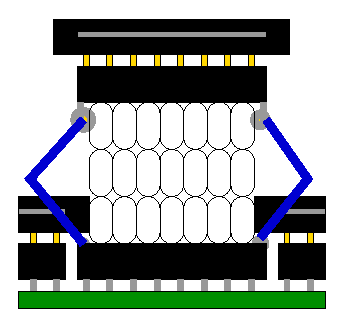
\epsfig{file=figures/cable_loft.eps,width=1.75in}
\caption{Lofting the cable connector (workaround).}
\label{figure:cableloft}
\end{center}
\end{figure*}

\begin{enumerate}
\item Take two 30-pin headers.  Cut off 4 10-pin lengths for
      the LED bargraph sockets.  (These need to be made out
      of the headers, so that it is possible to solder the
      sockets from the other side).  Solder these to the board.
      Place a 20-pin socket temporarily into the headers to 
      keep them vertical while soldering.
\item Solder the 4 20-pin sockets on the back of the board.
      The one that comes up between the bargraph sockets is a bit tricky.
\item Take a 30-pin header and snip pins 10 and 20 off, plus trim off
      the 30th pin completely.  Repeat.  Solder into place as
      alphanumeric sockets.  Place a wide 24-pin socket across while
      soldering to keep vertical.
\item Cut 22 2-pin lengths of the 30-pin headers for LED sockets.
      Solder them in place; scotch tape can temporarily hold them.
\item Place all of the LED displays into their sockets.
      {\bf WORKAROUND} If you are using the
      Mark2 board the 12 red LEDs are indicated backwards, you'll
      have to install them opposite the way indicated on the PCB.
\item {\bf WORKAROUND} If you have the Mark2 board then the
      cable connectors are too close together to fit in the socket.
      As a workaround build a stack of cut up 30-pin headers 8 wide
      and place on the middle connector.
      Stack 3 high.  Then solder wires from the PCB up to the far right and 
      left pins of a 10-wide socket on top. This will allow the side 
      connectors to fit, as well as the middle one to be lofted.
      See Figure~\ref{figure:cableloft}.
\end{enumerate}



\begin{figure*}[tbp]
\begin{center}
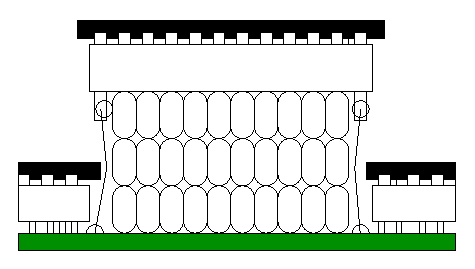
\epsfig{file=figures/chip_loft.eps,width=2.5in}
\caption{Lofting the chip socket (workaround).}
\label{figure:chiploft}
\end{center}
\end{figure*}


\section{Building the Logic Board}
\begin{enumerate}
\item Solder the sockets in place:  first the 4 24-pin wide ones, then
      the 4 20-pin sockets, finally the 1 16-pin socket.
\item You can optionally use parts of 30-pin header to make i2c and voltage
      interface sockets.
\item Bend the transistors down at a right angle (so they lie flush) 
      so that the cable headers can fit overtop.  Solder in place.
\item Solder the resistors in place.  
      {\bf WORKAROUND} The 27K resistor is mislabeled
      21K on the board.  3.3K = Orange Orange Red. 
      4.7K = Yellow Violet Red.  16K = Brown Blue Orange.
      27K = Red Violet Orange.
\item Solder the capacitors in place.
\item Solder the power socket.
\item Solder on the parallel connector.
\item {\bf WORKAROUND} Loft the middle SAA1064 chip socket.  Use two 10-wide
      headers to loft it.  Then solder wires to the holes on either
      end and loft.  You might insert heat-shrink tubing around wires
      to keep shorts from happening.  See Figure~\ref{figure:chiploft}.
\item Insert the 74HC05 chip and the four SAA1064 chips.

\end{enumerate}

\pagebreak

\section{Assembling the Whole Thing}
\begin{enumerate}
\item {\bf WORKAROUND} If the left side of the board won't fit in the
      case due to the case screw channel, you'll need to file a 
      semi-circular hole so that the board will fit.
\item Screw the logic board to base using two of the screws that
      came with the case.
\item Crimp the 4 cables with 20-pin connectors on either end.
      A crimper really helps here, and you really need one that
      has a DIP crimping substrate (hard to find).
      From the front, the left cable is 5in, next 2.5in (longer
      if you don't need the workaround), 3in, then 5.5in.      
\item Connect cables.  {\bf WORKAROUND}  If using mark1 logic board,
      need to trim the side off of the right-side connector
      so it can fit and not conflict with bottom right connector.
\item Plug in 5V adapter and parallel port.  Test using one
      of the sample programs.
\end{enumerate}

\section{Testing}
\begin{enumerate}
\item Before inserting ICs, apply 5V power and check that power is
      at proper pins.
\item Try inserting SAA1064s one at a time and then running sample
      programs to make sure each works/no problems before inserting all.
\end{enumerate}

\pagebreak




\section{Optional USB Board}


\subsection{USB Parts List}

\begin{tabular}{|c|l|c|c|}
\hline
Part No   &  Description    &  Quantity    &   Source \\
\hline
\hline
          &  USBtiny AVR Programmer  & 1  & adafruit\\ %$22
\hline
\hline
          &  Proto Board             & 1  & ????    \\ %got long ago
          &  Male 6-pin header       & 1  & Jameco 115035 \\ % .29
          &  8-pin machine socket    & 1  & \\
\hline
\hline
          &  22pF capcaitor          & 2  & \\
          &  12MHz crystal           & 1  & \\
          &  ATTiny45                & 1  & \\
          &  68$\Omega$ Resistor          & 2  & \\
          &  2.2K Resistor           & 1  & \\
          &  3.6V Zener Diode        & 2  & \\
          &  10$\mu$F electrolytic cap   & 1  & \\
          &  100nF (.1$\mu$F) cap        & 1  & \\
          &  10K Resistor            & 2  & \\
          &  USB B connector         & 1  & \\
          &  6-foot USB cable        & 1  & \\
          &  8-pin machine socket    & 1  & \\
          &  Perf Board              & 1  & Radio Shack 276-159B \\
\hline

\hline
\end{tabular}

\subsection{USB AVR Programming Board}

\begin{figure*}[tbp]
\begin{center}
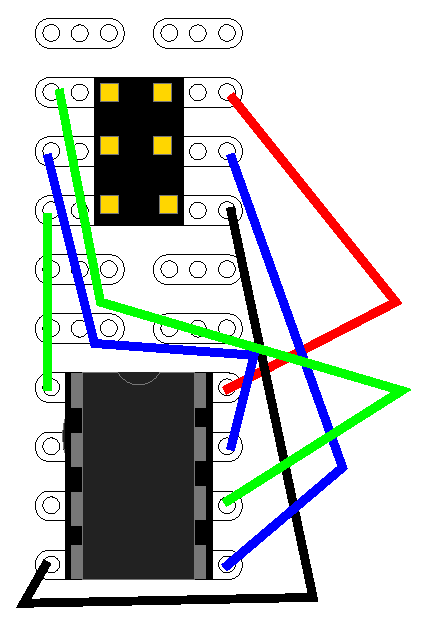
\epsfig{file=figures/usb_flash.eps,width=2in}
\caption{Setup for flashing ATTINY45 with USB-tiny-ISP}
\label{figure:avrprog}
\end{center}
\end{figure*}

\begin{enumerate}
\item First we need to flash the ATTINY45.  Get an AVR programmer
I used the USBtinyISP, from {\tt http://www.ladyada.net/make/usbtinyisp/}
\item You'll need to set wire up an adapter so the pins from the 
programmer go to the right pins of the ATTINY45.  The one I made used
some existing perf board I had, and can be seen in Figure~\ref{figure:avrprog}
\end{enumerate}

\pagebreak

\subsection{Flashing the ATTINY45}

This assumes you are using USBtinyISP.
\begin{enumerate}
\item Jumper the USBtinyISP to provide USB power.
\item Insert ATTINY45 into the board, attach 6-pin jumper
      from USBtinyISP.
\item Plug the USBtinyISP into a USB port.  The green light
      should come on.
\item Use {\tt avrdude} to do the programming.  On Debian Linux
      you can do an {\tt apt-get install avrdude} to install.
\item Obtain the USB firmware.  Get this from the 
      i2c tiny USB page
      {\tt http://www.harbaum.org/till/i2c\_tiny\_usb/} or eventually
      I will include it here.
\item Program as so:\\
      {\tt avrdude -Pattiny45 -c usbtiny -U lfuse:w:0xdf:m 
       -U hfuse:w:0x5f:m -U flash:w:firmware.hex}
\end{enumerate}


\begin{figure*}[tbp]
\begin{center}
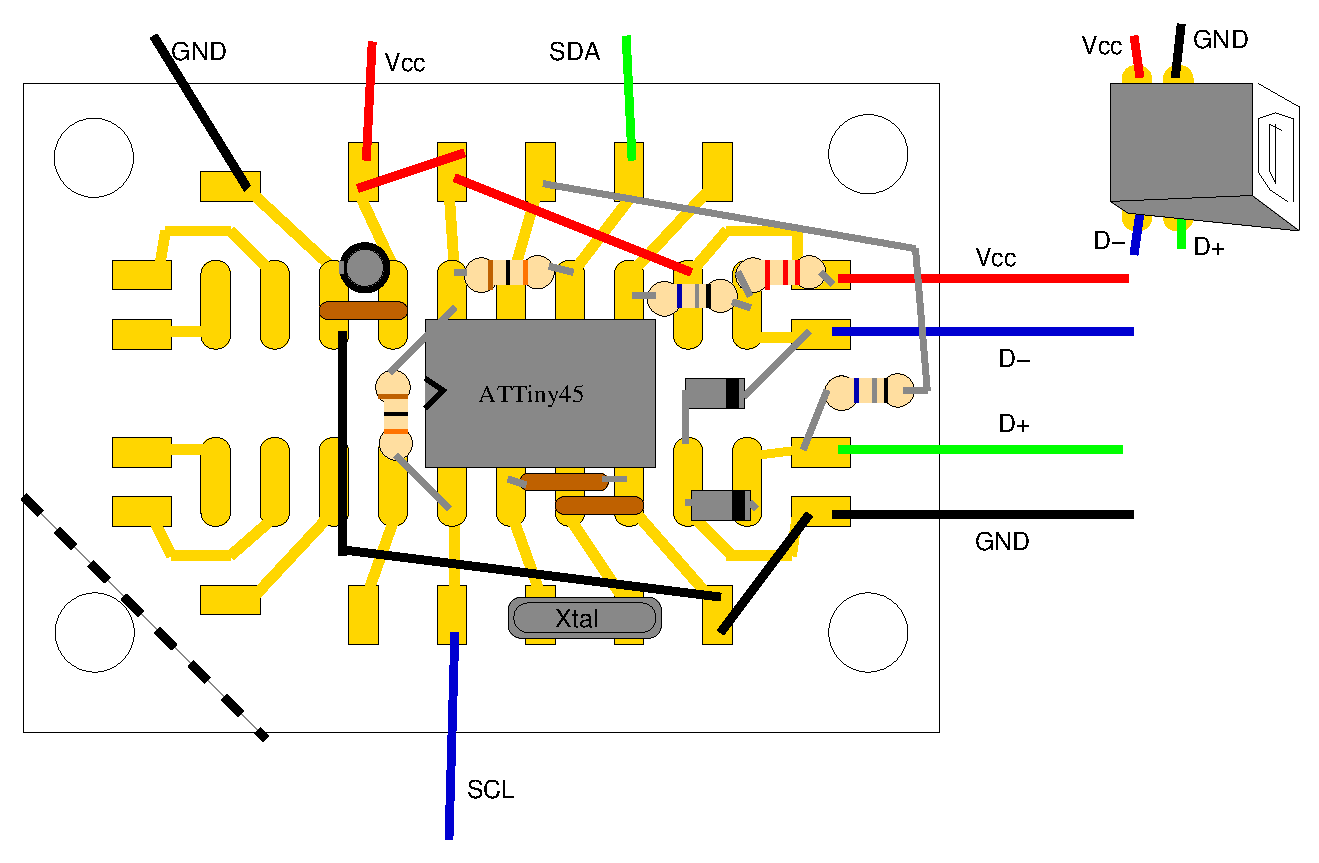
\epsfig{file=figures/usb_i2c.eps,width=4in}
\caption{Layout of USB to i2c board.}
\label{figure:usbi2c}
\end{center}
\end{figure*}

\subsection{USB to I2C Converter Board}

\end{document}
